% Drawing 69/01-11 -- folder 69, batch 01, archive page 13 (PDF page 14).
% Transcription: biffé, à gauche : $I$ et trois flèches parallèles marquées $i_3$, $i'_1$, $i_2$
% Kind: struck: I and three parallel arrows. Method 2 (schematic redraw from the facsimile). Status: partial.
% Notes: Struck through. I, and three parallel arrows rising to the right, marked i_3, i'_1, i_2 (letters read from the transcription; on the crop they are barely legible under the strike). Drawn grey.
% Coordinates: 1 unit = 1 mm = 1/100 of the crop width (bbox in page fractions: [0.1, 0.28, 0.45, 0.33]).
% Redrawn by Claude (claude-opus-5-5), issue #73, 2026-11-07; not checked by a human; not compiled (no TeX in the session).
% Rights: reproduces part of the work -- behind RENDER_TRANSCRIPTS, never published by itself.
\documentclass[tikz,border=3pt]{standalone}
\usepackage{amsmath,amssymb}
\usetikzlibrary{patterns,arrows.meta}
\tikzset{pencil/.style={black!45}, struck/.style={black!35}, mark/.style={circle,draw,inner sep=1.3pt}, pt/.style={circle,fill,inner sep=0.9pt}, opt/.style={circle,draw,fill=white,inner sep=1.1pt}}
\begin{document}
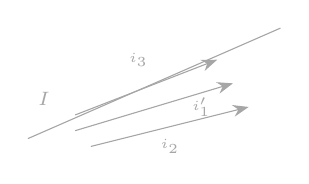
\begin{tikzpicture}[x=1mm,y=1mm,line cap=round,line join=round,font=\scriptsize]
\node[inner sep=1pt,struck] at (40,-13) {\scriptsize $I$};
\draw[-{Stealth[length=2mm]},struck] (44,-15) -- (62,-8);
\draw[-{Stealth[length=2mm]},struck] (44,-17) -- (64,-11);
\draw[-{Stealth[length=2mm]},struck] (46,-19) -- (66,-14);
\node[inner sep=1pt,struck] at (52,-8) {\tiny $i_3$};
\node[inner sep=1pt,struck] at (60,-14) {\tiny $i'_1$};
\node[inner sep=1pt,struck] at (56,-19) {\tiny $i_2$};
\draw[struck] (38,-18) -- (70,-4);
\end{tikzpicture}
\end{document}
